\documentclass[polish]{inz}

%+Make Index
\usepackage{makeidx}
\makeindex
%-Make Index

\usepackage{polski}
\usepackage[utf8]{inputenc}
\usepackage[OT4]{fontenc}

%+Title
\title{Graficzne interfejsy aplikacji opartych o biblioteki Qt i KDE}
\author{Jan J\k{e}drychowski\\\L{}ukasz Spas}
\date{2012}
\advisor{dr in\.{z}. Igor Wojnicki}
%-Title

\begin{document}
\maketitle

\chapter{Wstęp}

W dzisiejszych czasach coraz bardziej powszechne staje się wykorzystanie przeglądarek do zadań, do których wcześniej używane były duże aplikacje klienckie. Powstają rozwiązania, które starają się oddzielić logikę obliczeniową od warstwy prezentacji, przenosząc jednocześnie tę pierwszą na stronę serwera. Rozwój technologii HTML5 rozszerzającej standard o elementy canvas, websocket, webworkers i inne umożliwia tworzenie aplikacji o możliwościach takich samych jakie niegdyś były dostępne tylko w programach desktopowych. Co więcej gwarantuje międzyplatformowość nie tylko w rozumieniu softwareowym - jedna aplikacja dostępna jest zarówno na komputerach osobistych, tabletach, telefonach i innych urządzeniach wyposażonych w przeglądarkę.

W niektórych rozwiązaniach zastąpienie starych aplikacji desktopowych nowymi aplikacjami webowymi (przeglądarkowymi) jest jednak niemożliwe, czasochłonne lub zbyt kosztowne.

Podczas badań rynku pod kątem aktualnie dostępnych rozwiązań dostrzeżono braki w solucjach umożliwiających zdalną interakcję z pojedynczymi aplikacjami. Większość solucji dostępnych na rynku wymusza udostępnienie całego pulpitu oraz wymaga od użytkownika końcowego (klienta) posiadania odpowiedniego, nierzadko płatnego oprogramowania (np. TeamViewer, VNC, Citrix i inne). Celem projektu jest stworzenie alternatywy wymagającej od strony klienta jedynie przeglądarki obsługującej HTML5 bez konieczności instalacji jakichkolwiek pluginów (np. Java, Flash).

Głównym wzorcem dla tej pracy jest projekt GTK+ Broadway powstały w 2011 roku oferujący dostęp przez przeglądarkę internetową do aplikacji działających pod kontrolą biblioteki GTK na zdalnym serwerze. Do tej pory nie istniało rozwiązanie oferujące podobną funkcjonalność dla biblioteki QT i stworzony na potrzeby tej pracy projekt jest pierwszą taką implementacją.
Kluczowym czynnikiem wyróżniającym tę pracę na tle innych jest innowacyjny sposób przesyłu danych do wizualizacji okien i ich elementów, który nie opieraja się na transmisji bitmap.

\chapter{Podstawy teoretyczne}
W rodziale tym przedstawione zostaną najważniejsze informacje dotyczące technologii wykorzystanych w projekcie. 

\section{Szczegóły niektórych rozwiązań HTML5}
Text in section ...

\section{Opis biblioteki Qt}
W tym podrozdziale zostaną przedstawione mechanizmy biblioteki Qt wykorzystane przy tworzeniu projektu, o którym stanowi niniejsza praca. 

\subsection{System zdarzeń}


\subsection{System widgetów}


\subsection{System rysowania}
Rysowanie w bibliotece Qt standardowo zostało zaimplementowane jedynie dla rysowania na ekranie wykorzystując API systemu operacyjnego, dla którego Qt zostało skompilowane. Moduł rysowania jest niejako opakowaniem dla wywołań systemowych ujednolicając jego logikę i umożliwiając pełną przenośność aplikacji. Na rysunku \ref{paintsystem-core} przedstawiony został kaskadowy model systemu rysowania w Qt. 

Klasa QPaintDevice nie odnosi się bezpośrednio do logiki rysowania. Udostępnia ona jedynie informacje o typie urządzenia wyjściowego, na którym operował będą pozostałe klasy. Informacją taką jest na przykład jednostka miary odległości (pixel, punkt), rozmiar urządzenia (ekranu, papieru w drukarce) czy rodzaj obrazu wyjściowego (raster, bitmapa, grafika wektorowa). Dzięki tym informacjom pozostałe moduły mogą dostosować swoje działanie dla uzyskania maksymalnej efektywności.
 
Klasa QPainter udostępnia jednolity interfejs dla developerów umożliwjający rysowanie podstawowych obiektów takich jak: linie, kwadraty, okręgi, obrazy, etc. Klasa ta wykorzystuje następnie metody klasy QPaintEngine. 

\begin{figure}
  \centering
  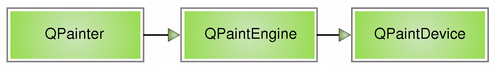
\includegraphics[width=\textwidth,height=!]{img/paintsystem-core.png}
  \caption{Schemat budowy systemu renderowania w bibliotece Qt}
  \label{paintsystem-core}
\end{figure}

\chapter{Określenie problemu i proponowane rozwiązanie}
Text in first chapter ...

\chapter{Implementacja}
Text in first chapter ...

\section{Po stronie serwera}
Text ...

\section{Po stronie klienta}
Text ...

\section{Napotkane problemy}
Text ...

\chapter{Testy aplikacji}
Text ...

\section{Testy w środowisku lokalnym}
Text ...

\section{Testy w sieci Internet}
Text ...

\chapter{Podsumowanie}
Text ...

%+Make Index
\printindex
%-Make Index

\end{document}